\documentclass{article}
\usepackage{spconf,amsmath,amssymb,amsfonts,graphicx,booktabs,multirow,array,cite,url,dblfloatfix,hyperref,tabularx,xcolor}
\hypersetup{hidelinks}
\newcolumntype{Y}{>{\centering\arraybackslash}X}
\newcolumntype{C}{>{\hsize=0.80\hsize\centering\arraybackslash}X}
\newcolumntype{W}{>{\hsize=1.24\hsize\centering\arraybackslash}X}

\def\x{{\mathbf x}}
\def\L{{\cal L}}

\title{HESOD: High-Resolution Efficient Small Object Detection via Semantic-Spectral Dual Selection}

% ICASSP 2027 does not perform blind review (confirmed via the official
% Paper-kit.md), so the author list is included directly. Superscript
% numbers on \name map each author to their \address line; $^{\dagger}$
% marks co-first authors (Jiawei Zhong, Sicheng Xu), footnoted via a
% plain \thanks{} on the first \dagger-marked name (empirically confirmed
% 2026-09-xx: spconf.sty's \thanks{} DOES auto-print a leading footnote
% mark despite its own doc comment claiming otherwise -- do not also
% hand-type a matching symbol inside the \thanks{} text, or it doubles up,
% e.g. "$^\dagger$$^\dagger$"). $^{\ast}$ (via \sthanks, same
% auto-mark behavior, intentionally relied on) marks the corresponding
% author (Hui Zhang). Neither symbol is an official ICASSP/Paper-kit
% field -- both are informal, widely-used academic conventions.
\name{Jiawei Zhong$^{1,\dagger}$\thanks{Source code at \url{https://github.com/deepsota-ai/HESOD}.}\thanks{These authors contributed equally to this work.}, Sicheng Xu$^{2,\dagger}$, Dandan Liu$^{3}$, Hui Zhang$^{2}$\sthanks{Corresponding author.}}
\address{
  $^{1}$DeepSOTA AI, San Jose, CA, USA \\
  $^{2}$College of Information, Mechanical and Electrical Engineering, Shanghai Normal University, China \\
  $^{3}$College of Electronics and Information Engineering, Shanghai University of Electric Power, China
}

% Spacing tweaks for tight 4+1 page layout
\setlength{\floatsep}{4pt plus 1pt minus 1pt}
\setlength{\textfloatsep}{4pt plus 1pt minus 1pt}
\setlength{\dblfloatsep}{4pt plus 1pt minus 1pt}
\setlength{\dbltextfloatsep}{4pt plus 1pt minus 1pt}
\setlength{\intextsep}{4pt plus 1pt minus 1pt}
\setlength{\abovecaptionskip}{2pt}
\setlength{\belowcaptionskip}{1pt}
\setlength{\skip\footins}{5pt plus 1pt minus 1pt}
\setlength{\abovedisplayskip}{2pt plus 1pt minus 1pt}
\setlength{\belowdisplayskip}{2pt plus 1pt minus 1pt}
\setlength{\abovedisplayshortskip}{1.0pt plus 1pt}
\setlength{\belowdisplayshortskip}{1.0pt plus 1pt minus 1pt}

% Float placement flexibility
\renewcommand{\topfraction}{0.95}
\renewcommand{\bottomfraction}{0.95}
\renewcommand{\textfraction}{0.05}
\renewcommand{\floatpagefraction}{0.85}
\renewcommand{\dbltopfraction}{0.95}
\renewcommand{\dblfloatpagefraction}{0.85}

\begin{document}
\ninept
\raggedbottom
\setlength{\abovedisplayskip}{2pt plus 1pt minus 1pt}
\setlength{\belowdisplayskip}{2pt plus 1pt minus 1pt}
\setlength{\abovedisplayshortskip}{1.0pt plus 1pt}
\setlength{\belowdisplayshortskip}{1.0pt plus 1pt minus 1pt}
\maketitle

\begin{abstract}
Tiny-object detection in high-resolution aerial and maritime imagery must contend with vast, redundant backgrounds and extreme scale variation. While spatial selective computation routes foreground regions to cut latency, existing single-evidence selectors suffer severe semantic collapse on micro targets, causing irrecoverable pruning. We propose \textbf{HESOD} (\textbf{H}igh-Resolution \textbf{E}fficient \textbf{S}mall \textbf{O}bject \textbf{D}etection), a dual-evidence framework unifying semantic-spectral routing, coverage-constrained optimization, and lightweight detection. HESOD couples semantic objectness with constant-width spectral saliency under a monotonic evidence-preserving max-fusion rule to rescue degraded targets. An object-level soft-coverage loss optimizes multi-cell instance coverage across ground-truth objects for recall-safe routing. To recover downstream efficiency, an Inverse-Residual Shared-Parameter Partial-Convolution (ISPP) head compresses parameters by \textgreater27\% with only fractional FLOPs overhead. Experiments show that HESOD improves $\mathrm{mAP@.5}$ by 0.9\,pp and 2.3\,pp (boosting total instance recall by 3.66\,pp and 3.33\,pp) on UAVDT and SeaPerson, respectively, at up to 106 FPS, making it well suited to resource-constrained deployment.
\end{abstract}

\begin{keywords}
Small object detection, selective computation, spectral saliency, coverage optimization, UAV
\end{keywords}

\section{Introduction}
\label{sec:intro}

High-resolution aerial and maritime vision is fundamental to intelligent surveillance, environmental monitoring, and search-and-rescue. In operational scenarios across aerial and maritime domains~\cite{VisDrone,UAVDT,TinyPerson}, targets of interest typically occupy only a handful of pixels (\textless$16\times16$\,px) amid massive uniform backgrounds (\textgreater70\%--80\%)~\cite{AutoFocus}. Evaluating standard dense deep detectors across multi-megapixel grids ($1280\times 1280$ to $2048\times 2048$) incurs prohibitive arithmetic latency on resource-constrained platforms.

To eliminate redundant computation, \emph{spatial selective computation} routes feature processing to prospective foreground regions~\cite{QueryDet,CEASC}. Notably, ESOD~\cite{ESOD} predicts an early spatial priority heatmap after a shallow stem, slicing features into candidate patches (AdaSlicer) and bypassing background across downstream stages.

\begin{figure}[!t]
\centering
% Column headers
\begin{minipage}[b]{0.036\columnwidth}\hfill\end{minipage}\hspace{1mm}%
\begin{minipage}[b]{0.468\columnwidth}
  \centering
  \scriptsize\textbf{UAVDT (\emph{Urban})}\\[-0.2mm]
  \scriptsize img000015
\end{minipage}\hspace{1.2mm}%
\begin{minipage}[b]{0.468\columnwidth}
  \centering
  \scriptsize\textbf{SeaPerson (\emph{Surfing})}\\[-0.2mm]
  \scriptsize rgb\_x0080\_P000\_115344
\end{minipage}

\vspace{0.2mm}
% Row 1: Ground Truth
\begin{minipage}[c]{0.036\columnwidth}
  \centering
  \rotatebox{90}{\scriptsize\textbf{(a) Ground Truth}}
\end{minipage}\hspace{1mm}%
\begin{minipage}[c]{0.468\columnwidth}
  \centering
  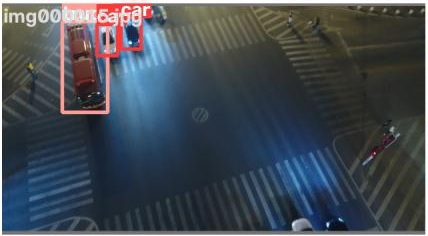
\includegraphics[width=\linewidth]{figures/uavdt-img000015/img000015-label.jpg}
\end{minipage}\hspace{1.2mm}%
\begin{minipage}[c]{0.468\columnwidth}
  \centering
  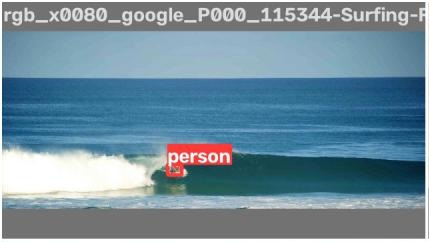
\includegraphics[width=\linewidth]{figures/rgb-x0080-google-115344/rgb-x0080-google-115344-Surfing-label.jpg}
\end{minipage}

\vspace{0.4mm}
% Row 2: ESOD (Baseline)
\begin{minipage}[c]{0.036\columnwidth}
  \centering
  \rotatebox{90}{\scriptsize\textbf{(b) ESOD}}
\end{minipage}\hspace{1mm}%
\begin{minipage}[c]{0.468\columnwidth}
  \centering
  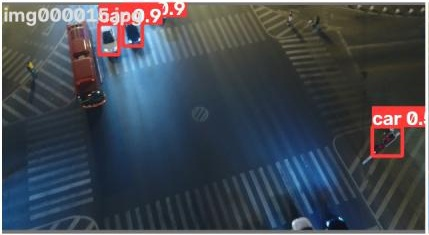
\includegraphics[width=\linewidth]{figures/uavdt-img000015/img000015-esod.jpg}
\end{minipage}\hspace{1.2mm}%
\begin{minipage}[c]{0.468\columnwidth}
  \centering
  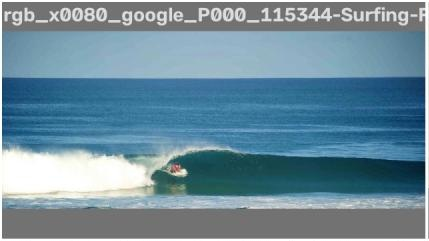
\includegraphics[width=\linewidth]{figures/rgb-x0080-google-115344/rgb-x0080-google-115344-Surfing-esod.jpg}
\end{minipage}

\vspace{0.4mm}
% Row 3: HESOD (Ours)
\begin{minipage}[c]{0.036\columnwidth}
  \centering
  \rotatebox{90}{\scriptsize\textbf{(c) HESOD}}
\end{minipage}\hspace{1mm}%
\begin{minipage}[c]{0.468\columnwidth}
  \centering
  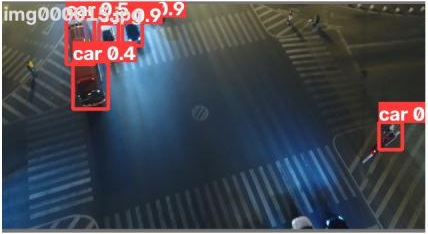
\includegraphics[width=\linewidth]{figures/uavdt-img000015/img000015-hesod.jpg}
\end{minipage}\hspace{1.2mm}%
\begin{minipage}[c]{0.468\columnwidth}
  \centering
  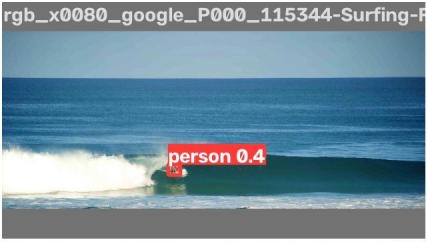
\includegraphics[width=\linewidth]{figures/rgb-x0080-google-115344/rgb-x0080-google-115344-Surfing-hesod.jpg}
\end{minipage}
\vspace{-2.5mm}
\caption{Visual comparison on UAVDT and SeaPerson. Baseline ESOD drops micro targets (b), while HESOD restores full instance recall (c).}
\label{fig:teaser}
\end{figure}

However, spatial selection operates under a severe \emph{asymmetric error cost}: false-positive background patches merely incur minor compute overhead, whereas discarding a true tiny target produces an \emph{irrecoverable false negative}. Existing detectors rely on single semantic objectness with independent per-cell BCE. Under extreme downsampling, micro targets suffer severe semantic collapse, causing faint instances to be prematurely pruned (Fig.~\ref{fig:teaser}(b)). To overcome this recall dilemma, we observe that tiny targets retain high-frequency spatial gradients and spectral saliency even when deep semantics fade~\cite{SET,Guo2025DualDomain,Zhao2025TGRS}. We then propose High-Resolution Efficient Small Object Detection (\textbf{HESOD}) to establish recall-safe, evidence-preserving sparse routing. By coupling dual-evidence routing with an object-level soft-coverage loss, our selector reliably rescues these dropped targets (Fig.~\ref{fig:teaser}(c)). Our contributions include:
\begin{enumerate}\setlength{\itemsep}{0pt}\setlength{\parskip}{0pt}\setlength{\topsep}{1pt}
    \item \textbf{Dual-Evidence Spatial Routing}: We uncover single-semantic routers' vulnerability to feature collapse, coupling semantic objectness with constant-width gradient filtering for scale-robust structural priors independent of backbone capacity.
    \item \textbf{Evidence Preservation and Soft Coverage}: We formulate a monotonic max-fusion rule preventing multi-cue evidence dilution, paired with an object-level noisy-OR soft-coverage loss directly optimizing joint instance recall.
    \item \textbf{Compute Compensation and Empirical Gains}: We co-design an ISPP head that reduces detector parameters by \textgreater27\% while improving $\mathrm{mAP@.5}$ by 0.9/2.3\,pp on UAVDT and SeaPerson, boosting total instance recall by 3.66/3.33\,pp.
\end{enumerate}

\begin{figure*}[t]
\centering
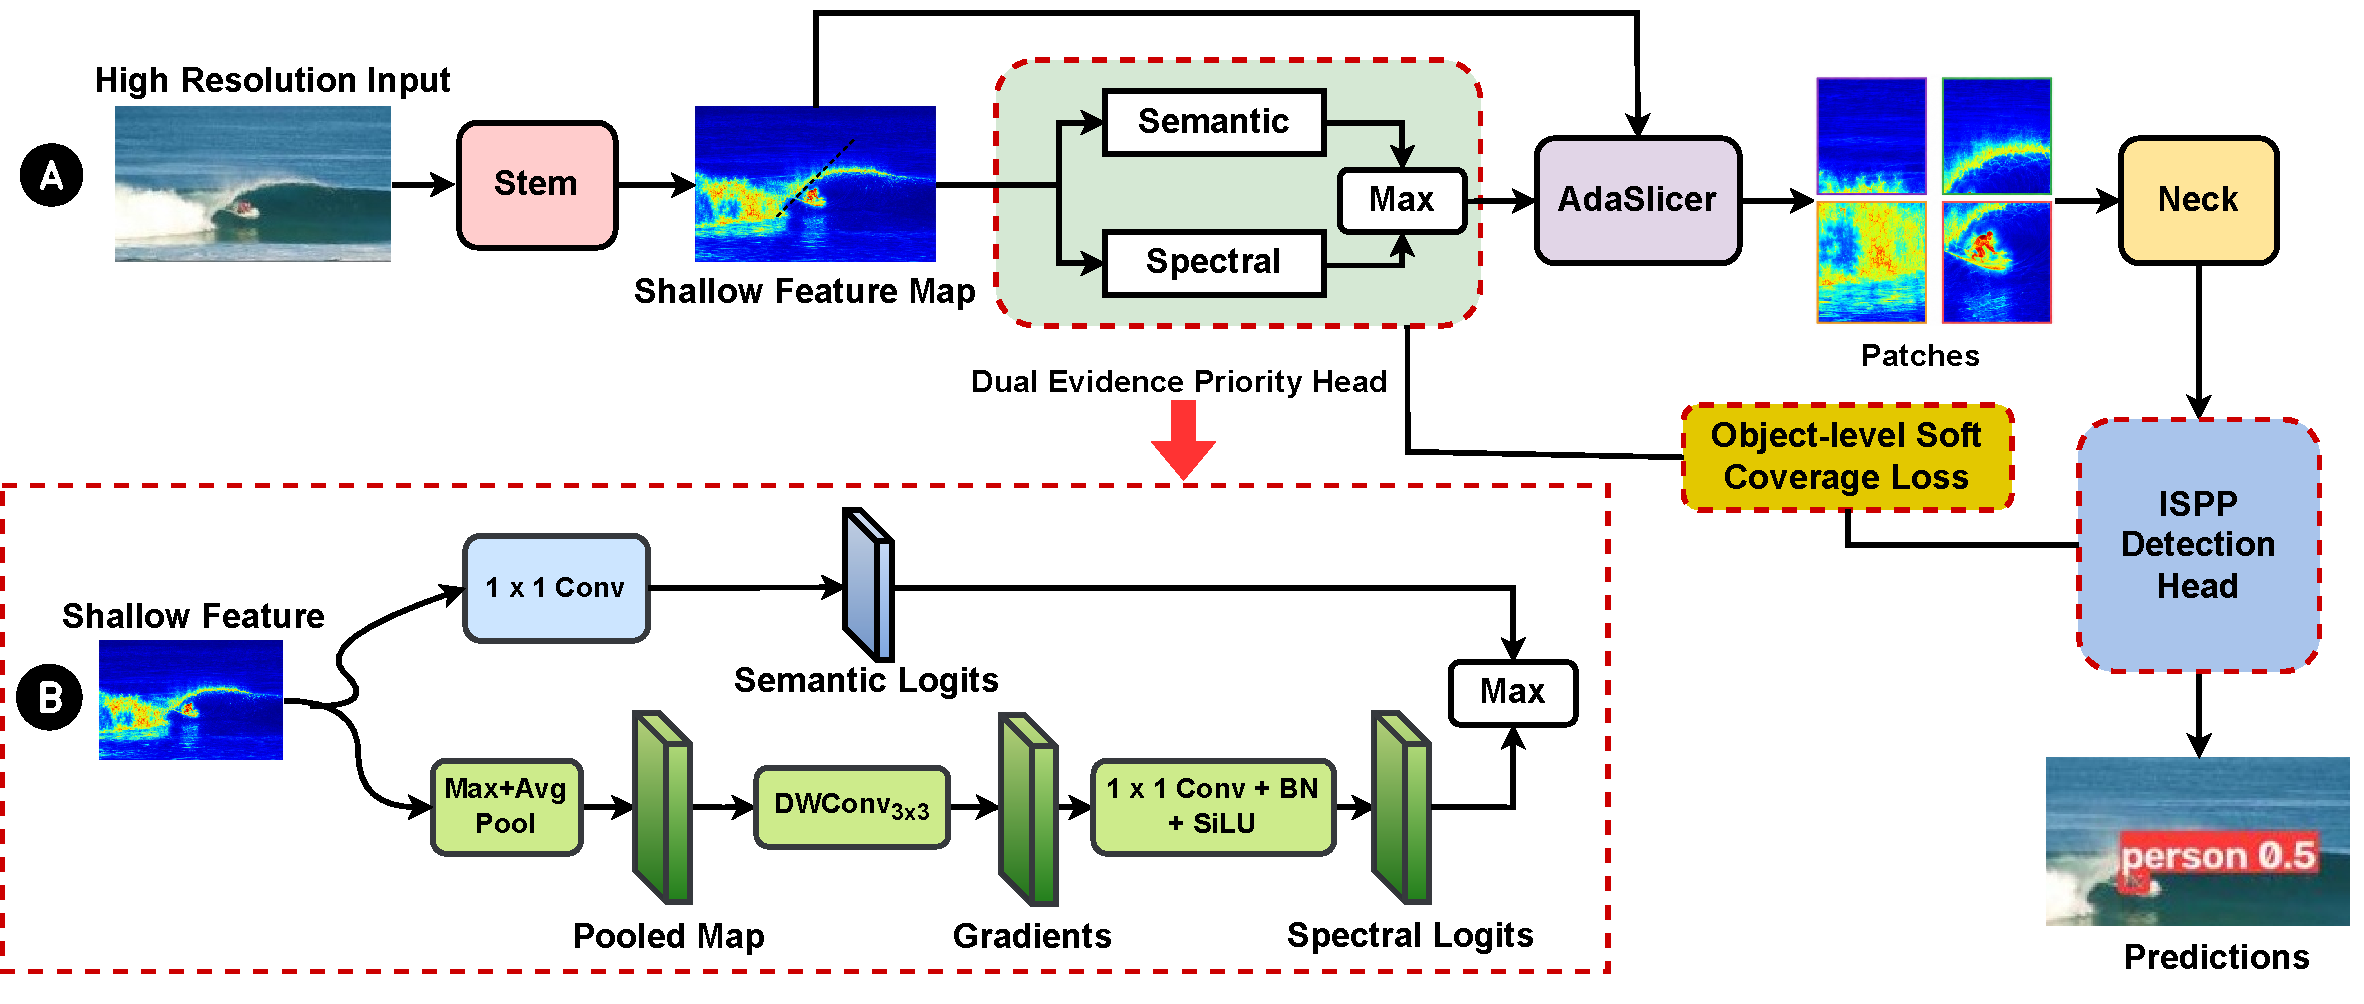
\includegraphics[width=0.90\textwidth]{figures/HESOD.pdf}
\vspace{-2.5mm}
\caption{Overview of HESOD: (a) End-to-end selective pipeline; (b) Dual-Evidence Priority Head. Red dashed boxes highlight our proposed contributions over ESOD.}
\label{fig:overview}
\end{figure*}

\section{Related Work}
\label{sec:related}

\subsection{Small Object Detection in High-Resolution Vision}
\label{ssec:related_sod}

Detecting tiny targets in high-resolution aerial and maritime imagery is severely challenged by extreme scale disparity, low contrast, and massive background areas ($>70\%\text{--}80\%$)~\cite{VisDrone,UAVDT,TinyPerson,SeaDronesSee}. Classical approaches utilize density-guided cropping (ClusDet~\cite{ClusDet}, DMNet~\cite{DMNet}) or scale-adaptive label assignment (NWD~\cite{NWD}, RFLA~\cite{RFLA}). Recently, ResBiDet~\cite{ResBiDet} introduced a coarse-to-fine framework using global heatmap guidance for region cropping. However, it relies on multi-scale image-level slicing and boundary stitching. In contrast, HESOD performs early feature-level selective routing directly within the detector trunk and explicitly optimizes instance coverage under irreversible pruning.

\subsection{Selective and Dynamic Computation}
\label{ssec:related_selective}

Dynamic computation accelerates inference by allocating compute strictly to prospective foreground regions (e.g., AutoFocus~\cite{AutoFocus}, QueryDet~\cite{QueryDet}, CEASC~\cite{CEASC}, and sparse location activation~\cite{Li2025Sparse}). Recently, coarse-to-fine detectors such as ESOD~\cite{ESOD} and OSDT~\cite{Wang2026OSDT} predict early spatial priority heatmaps to extract candidate patches. However, existing selectors rely exclusively on a single semantic score supervised by independent per-cell BCE. Under extreme scale disparity, micro targets suffer from semantic feature collapse after downsampling; meanwhile, per-cell BCE lacks joint instance-level coverage constraints, causing fatal false negatives under an asymmetric error cost. HESOD resolves this by combining semantic and spectral dual cues with object-level soft-coverage optimization.

\subsection{Spectral Saliency and Frequency Methods}
\label{ssec:related_spectral}

High-frequency edge gradients persist for micro targets even as photometric semantics fade~\cite{SET,Zhao2025TGRS}; recent methods exploit this via dense frequency transforms~\cite{SET}, frequency-gradient networks~\cite{Zhao2025TGRS}, dual-domain alignment~\cite{Guo2025DualDomain}, or multi-scale compensation~\cite{Wang2026HighFreq}, but all apply spectral cues \emph{downstream}, incurring substantial latency. In sharp contrast, HESOD repurposes high-frequency gradient saliency \emph{upstream} as an ultra-lightweight routing cue: channel pooling compresses stem features to 2 channels, enabling directional Laplacian and Sobel gradient filtering at constant width.



\section{Proposed Method}
\label{sec:method}

The architecture of HESOD is shown in Fig.~\ref{fig:overview}. From input $\mathbf{I} \in \mathbb{R}^{H \times W \times 3}$, a shallow stem extracts dense features $\mathbf{F} \in \mathbb{R}^{H_s \times W_s \times C}$. The \emph{Dual-Evidence Spatial Selector} then coordinates: (i) a priority head fusing semantic objectness with channel-pooled spectral saliency (Fig.~\ref{fig:overview}(b)) into spatial priority map $\mathbf{S} \in [0, 1]^{H_s \times W_s}$; and (ii) an AdaSlicer module (unchanged from ESOD~\cite{ESOD}) clustering candidate foreground cells into bounding patches $\mathcal{P}$. Downstream backbone stages and lightweight decoupled heads evaluate only retained patches $\mathcal{P}$, trained under the soft-coverage supervision (Sec.~\ref{ssec:coverage}) via the two-stage protocol (Sec.~\ref{ssec:head}).

\subsection{Dual-Evidence Priority Estimation}
\label{ssec:evidence}

To rescue micro targets with degraded semantic activations, HESOD couples high-level semantic confidence with low-level structural gradient saliency at negligible compute overhead (Fig.~\ref{fig:overview}(b)).

Let $\mathbf{f}_i \in \mathbb{R}^C$ denote the feature vector at spatial location $i$ in $\mathbf{F}$. The semantic branch predicts class-specific logits via a $1\times 1$ convolution: $\mathbf{z}^{\mathrm{sem}}_i = \mathrm{Conv}_{1\times 1}(\mathbf{f}_i) \in \mathbb{R}^{N_c}$. In parallel, the spectral branch extracts high-frequency structural gradients by first compressing channels via max- and mean-pooling:
\begin{equation}
\mathbf{F}_{\mathrm{pooled}} = \left[ \max_c \mathbf{F}_{:,:,c} \,\|\, \frac{1}{C}\sum_{c=1}^C \mathbf{F}_{:,:,c} \right] \in \mathbb{R}^{H_s \times W_s \times 2},
\label{eq:channel_pool}
\end{equation}
where $\mathbf{F}_{:,:,c} \in \mathbb{R}^{H_s \times W_s}$ is the $c$-th channel of $\mathbf{F}$ and $\|$ denotes channel-wise concatenation. Compressing $\mathbf{F}$ to 2 channels retains peak edge activation and background energy, after which a learnable depthwise $3\times 3$ convolution bank---initialized with discrete Laplacian and directional Sobel operators---filters $\mathbf{F}_{\mathrm{pooled}}$ into 6 structural channels at $\mathcal{O}(H_s W_s)$ cost independent of width $C$. In the 2D spatial frequency domain, the discrete Laplacian is approximately isotropic in the low-frequency limit, with $|H(\mathbf{\omega})| \propto \|\mathbf{\omega}\|^2$, naturally amplifying edge transitions. Because micro targets (\textless$16^2$\,px) manifest as localized high-frequency spatial impulses whose gradient energy resists downsampling~\cite{Zhao2025TGRS}, this branch supplies a constant-width prior independent of deep semantic capacity. A $1\times 1$ projection maps features to $N_c$, yielding spectral logits $\mathbf{z}^{\mathrm{spec}}_i \in \mathbb{R}^{N_c}$.

To prevent confidence dilution on faint targets, evidence fusion enforces \emph{evidence preservation}. Linear combinations risk destructive interference: an unconfident or negative activation in one branch can drag down a confident signal in the other below the routing threshold. Instead, we formulate a parameter-free elementwise maximum:
\begin{equation}
z_{i,c} = \max\!\left(z^{\mathrm{sem}}_{i,c},\, z^{\mathrm{spec}}_{i,c}\right), \quad s_i = \max_{c=1}^{N_c} \sigma(z_{i,c}),
\label{eq:fusion}
\end{equation}
This operation functions as an evidence-preserving OR gate: since $z_{i,c} \ge z^{\mathrm{sem}}_{i,c}$ and $z_{i,c} \ge z^{\mathrm{spec}}_{i,c}$, neither branch can ever suppress genuine candidate cues. Cells with priority $s_i > \tau$ are clustered into bounding patches $\mathcal{P}$ for downstream detection.

\subsection{Object-Level Soft-Coverage Loss}
\label{ssec:coverage}

Standard pixel-wise binary cross-entropy (BCE) evaluates grid cells independently, failing to guarantee instance-level coverage: a selector may over-allocate cells to large objects while dropping micro objects whose receptive fields contain only weak responses. To prevent premature false negatives, we formulate a differentiable object-level soft-coverage loss.

Let $\mathcal{N}(j)$ denote the set of selector cells overlapping ground-truth box $j \in \{1, \dots, N_{\mathrm{gt}}\}$. We formulate a noisy-OR differentiable coverage surrogate and its weighted instance loss:
\begin{equation}
p_j^{\mathrm{cover}} = 1 - \prod_{i \in \mathcal{N}(j)} (1 - s_i), \quad \ell_j = -w_j \log\left( p_j^{\mathrm{cover}} + \epsilon \right),
\label{eq:cover_loss}
\end{equation}
where $w_j = \operatorname{clip}(4/a_j, 1, 5)$ is a scale-adaptive weight based on bounding box area $a_j$ in cells, penalizing misses on micro targets ($a_j < 4$). For any cell $i \in \mathcal{N}(j)$, the gradient of $\ell_j$ with respect to cell score $s_i$ is:
\begin{equation}
\frac{\partial \ell_j}{\partial s_i} = -\frac{w_j}{p_j^{\mathrm{cover}} + \epsilon} \prod_{k \in \mathcal{N}(j) \setminus \{i\}} (1 - s_k).
\label{eq:cover_grad}
\end{equation}
When neighboring candidate cells have low scores ($s_k \to 0$), the product term approaches $1$, generating a strong gradient to boost cell $i$ and encouraging at least one cell to activate per instance. The overall soft-coverage loss averages over instances: $\mathcal{L}_{\mathrm{cover}} = \frac{1}{N_{\mathrm{gt}}} \sum_{j=1}^{N_{\mathrm{gt}}} \ell_j$. The multi-task training objective is $\mathcal{L} = \mathcal{L}_{\mathrm{det}} + \lambda_{\mathrm{sel}}(\mathcal{L}_{\mathrm{BCE}} + \lambda_{\mathrm{cov}}\mathcal{L}_{\mathrm{cover}})$, where $\mathcal{L}_{\mathrm{BCE}}$ is the per-cell selector BCE over scores $s_i$, with $\lambda_{\mathrm{sel}}=0.2$ and $\lambda_{\mathrm{cov}}=0.5$.

\subsection{Lightweight Decoupled Head and Training Protocol}
\label{ssec:head}

\begin{figure}[t]
\centering
\vspace{-1mm}
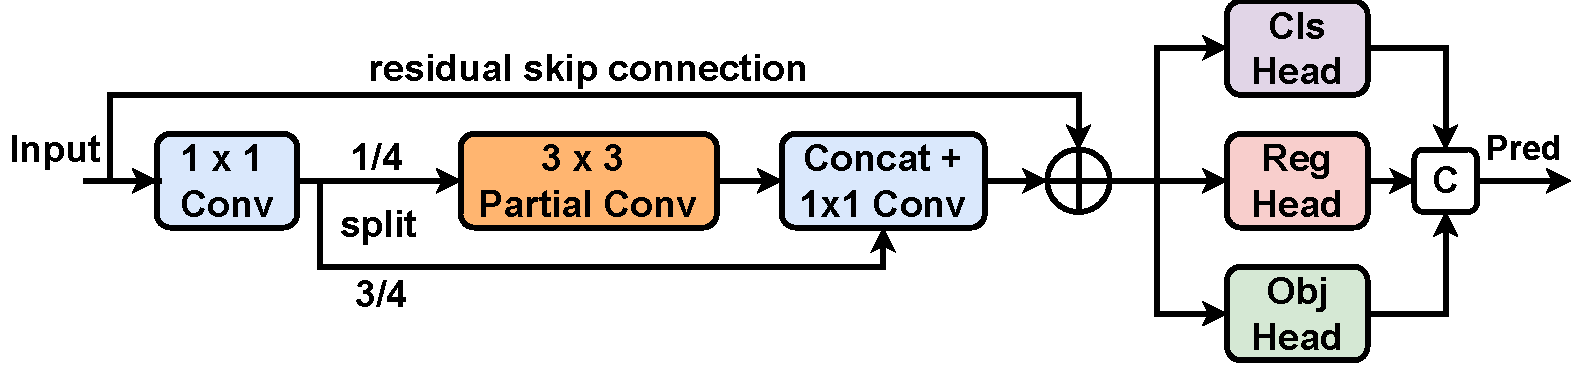
\includegraphics[width=\columnwidth]{figures/ISPPHead.pdf}
\vspace{-6mm}
\caption{Inverse-Residual Shared-Parameter Partial-Convolution (ISPP) Head (\textcircled{\scriptsize C} denotes channel concatenation).}
\label{fig:ispphead}
\vspace{7pt}
\end{figure}

While dual-evidence routing substantially improves patch coverage by retaining faint foreground regions, evaluating more candidate patches increases downstream detector computation. To recover this overhead without sacrificing selector gains, HESOD incorporates an ISPP decoupled head~\cite{ESODYOLO} as a dedicated compute compensator.

As shown in Fig.~\ref{fig:ispphead}, the ISPP head expands neck feature channels of width $C_1$ to $2C_1$, partitioning them into an active branch ($0.25$ ratio) processed by a $3\times 3$ Partial Convolution (PConv) and an identity passthrough branch ($0.75$ ratio). After linear projection and residual addition, decoupled $1\times 1$ heads predict classification, box regression, and objectness independently, lowering arithmetic complexity while eliminating inter-task gradient interference.

\textbf{Two-Stage Training Protocol.} To ensure stable routing behavior, HESOD employs a two-stage training scheme: (i)~\emph{Stage 1 (Selector Convergence)}: Train the Dual-Max selector with a coupled head under $\mathcal{L}_{\mathrm{cover}}$, establishing a well-calibrated priority heatmap; and (ii)~\emph{Stage 2 (Head Fine-Tuning)}: Freeze the upstream trunk (backbone, dual branches, router) and fine-tune the lightweight ISPP neck and decoupled heads on the frozen routing distribution. Relative to the uncompressed Dual-Max selector, this lightweight head slashes GFLOPs by 16.9\% and parameters by 27.5\% (on UAVDT) while fully preserving peak selector coverage (0.940), maintaining competitive real-time FPS with only fractional FLOPs overhead vs.~ESOD.


\section{Experiments}
\label{sec:experiments}

\subsection{Experiment Settings}
\label{ssec:settings}

We evaluate HESOD on two demanding high-resolution small-object benchmarks: \textbf{UAVDT}~\cite{UAVDT} ($1280 \times 1280\text{ px}$, urban vehicle surveillance across 3 classes) and \textbf{SeaPerson}~\cite{TinyPerson,SeaDronesSee} ($2048 \times 2048\text{ px}$, maritime search-and-rescue with $>85\%$ micro targets $<32\text{ px}$). Both evaluate full-resolution images without artificial cropping.

Selective detectors (ESOD family and our ablations) employ YOLOv5m backbones in PyTorch 2.8 trained for 50 epochs under selective protocols~\cite{ESOD}; HESOD trains the selector in Stage 1 and fine-tunes the lightweight ISPP head with the frozen selector in Stage 2. Dense and query baselines (Faster R-CNN, RetinaNet, QueryDet) retain canonical ResNet-50-FPN backbones, evaluated on identical test splits and resolutions. All models are benchmarked on an NVIDIA RTX 5090 GPU. Metrics include COCO $\mathrm{mAP@.5}$, scale-stratified recall across bins (\emph{Very Tiny} $<16^2$, \emph{Tiny} $16^2\text{--}32^2$, \emph{Small} $32^2\text{--}96^2$), and \emph{Bounding Patch Recall} ($\mathrm{BPR} = N_{\mathrm{cov}} / N_{\mathrm{gt}}$, where a target is covered if $|\mathrm{GT} \cap \mathcal{P}| / |\mathrm{GT}| > 0.5$ by selected patches $\mathcal{P}$).

\subsection{Main Benchmark Comparisons}
\label{ssec:main_results}

\begin{table}[t]
\centering
\caption{Benchmark results on UAVDT and SeaPerson.}
\label{tab:main_results}
\scriptsize
\setlength{\tabcolsep}{0pt}
\renewcommand{\arraystretch}{1.02}
\begin{tabular*}{\columnwidth}{@{\extracolsep{\fill}}lcccccc@{}}
\toprule
\textbf{Method} & \textbf{mAP@.5} & \shortstack{\textbf{Params}\\\textbf{(M)}} & \textbf{GFLOPs} & \shortstack{\textbf{Total}\\\textbf{Recall}} & \textbf{BPR} & \textbf{FPS} \\
\midrule
\multicolumn{7}{l}{\textit{\textbf{UAVDT Benchmark ($1280\times 1280$)}}} \\
Faster R-CNN~\cite{FasterRCNN}     & 0.336 & 43.3 & 772.5 & 79.68\% & -- & 18.8 \\
RetinaNet~\cite{RetinaNet}           & 0.296 & 36.4 & 360.9 & 83.44\% & -- & 19.8 \\
QueryDet$^\dagger$~\cite{QueryDet}   & 0.257 & 39.3 & --$^\dagger$ & 41.89\% & -- & 21.1 \\
ESOD~\cite{ESOD}                     & \underline{0.385} & \underline{35.9} & \textbf{68.2} & \underline{85.17\%} & \underline{0.884} & \textbf{117.8} \\
\textbf{HESOD (Ours)}                & \textbf{0.394} & \textbf{26.0} & \underline{74.9} & \textbf{88.83\%} & \textbf{0.940} & \underline{106.1} \\
\textit{$\Delta$ vs. ESOD} & \textbf{+0.9\,pp} & \textbf{-27.5\%} & +9.8\% & \textbf{+3.66\,pp} & \textbf{+5.6\,pp} & -9.9\% \\
\midrule
\multicolumn{7}{l}{\textit{\textbf{SeaPerson Benchmark ($2048\times 2048$)}}} \\
Faster R-CNN~\cite{FasterRCNN}     & 0.551 & 43.3 & 1546.8 & 67.27\% & -- & 23.1 \\
RetinaNet~\cite{RetinaNet}         & 0.473 & 36.4 & 942.7  & 65.98\% & -- & 28.0 \\
QueryDet$^\dagger$~\cite{QueryDet} & 0.627 & 39.3 & --$^\dagger$ & 61.56\% & -- & 14.0 \\
ESOD~\cite{ESOD}                   & \underline{0.750} & \underline{35.8} & \textbf{202.4} & \underline{84.42\%} & \underline{0.947} & \textbf{85.7} \\
\textbf{HESOD (Ours)}              & \textbf{0.773} & \textbf{25.9} & \underline{208.5} & \textbf{87.75\%} & \textbf{0.991} & \underline{80.6} \\
\textit{$\Delta$ vs. ESOD} & \textbf{+2.3\,pp} & \textbf{-27.6\%} & +3.0\% & \textbf{+3.33\,pp} & \textbf{+4.4\,pp} & -6.0\% \\
\bottomrule
\end{tabular*}
\vspace{0.4mm}
\parbox{\columnwidth}{\scriptsize BPR: Bounding Patch Recall. \textbf{Bold}: best; \underline{underline}: second-best (selective models).\\
$^\dagger$QueryDet uses CSQ (dynamic sparse FLOPs unamenable to static profiling; dense query counterparts: 973.5 / 2539.0 GFLOPs at 12.5 / 10.6 FPS on UAVDT / SeaPerson).}
\vspace{0.5mm}
\end{table}

\begin{table*}[t]
\centering
\vspace{-1.5mm}
\caption{Module ablation, efficiency, and scale recall breakdown on UAVDT and SeaPerson.}
\label{tab:ablation_and_recall}
\scriptsize
\setlength{\tabcolsep}{1.8pt}
\renewcommand{\arraystretch}{1.00}
\begin{tabularx}{\textwidth}{l*{6}{C}*{5}{W}}
\toprule
 & \multicolumn{6}{c}{\textbf{Detection Accuracy and Computational Efficiency}} & \multicolumn{5}{c}{\textbf{Physical-Scale Recall Breakdown}} \\
\cmidrule(lr){2-7} \cmidrule(lr){8-12}
\textbf{Configuration} & \shortstack{\textbf{mAP}\\\textbf{@.5}} & \shortstack{\textbf{mAP}\\\textbf{@.5:.95}} & \textbf{BPR} & \shortstack{\textbf{Params}\\\textbf{(M)}} & \textbf{GFLOPs} & \textbf{FPS} & \shortstack{\textbf{Very Tiny}\\\textbf{($<16^2$)}} & \shortstack{\textbf{Tiny}\\\textbf{($16^2\text{--}32^2$)}} & \shortstack{\textbf{Small}\\\textbf{($32^2\text{--}96^2$)}} & \shortstack{\textbf{Med/Lrg}\\\textbf{($>96^2$)}} & \shortstack{\textbf{Total}\\\textbf{Recall}} \\
\midrule
\multicolumn{7}{l}{\textit{\textbf{UAVDT Benchmark ($1280\times 1280$)}}} & \scriptsize(74,375) & \scriptsize(206,015) & \scriptsize(86,282) & \scriptsize(7,325) & \scriptsize(373,997) \\
(1) ESOD Baseline$^*$        & 0.385 & 0.214 & 0.884 & 35.9 & \textbf{68.2} & \textbf{117.8} & 79.43\% & 84.21\% & 94.54\% & 59.78\% & 85.17\% \\
(2) Semantic-only            & 0.384 & \underline{0.217} & 0.906 & 35.9 & 75.0 & \underline{113.8} & 79.13\% & 83.91\% & 94.00\% & 59.95\% & 84.82\% \\
(3) Spectral-only            & 0.387 & 0.209 & \underline{0.942} & 36.0 & 93.7 & 102.3 & 82.43\% & 88.72\% & 96.66\% & \underline{66.80\%} & 88.87\% \\
(4) (3) + Channel-Pooled     & \underline{0.394} & 0.209 & \textbf{0.963} & 35.9 & 99.3 & 97.6 & \textbf{86.88\%} & \textbf{92.23\%} & \textbf{97.74\%} & 66.43\% & \textbf{91.93\%} \\
(5) Dual-Concat              & 0.371 & 0.205 & 0.919 & 35.9 & 83.9 & 107.2 & 79.09\% & 85.85\% & 95.85\% & 62.66\% & 86.35\% \\
(6) Dual-Max                 & \textbf{0.395} & \textbf{0.218} & 0.940 & 35.9 & 90.1 & 102.3 & \underline{85.69\%} & \underline{89.97\%} & \underline{97.37\%} & 65.99\% & \underline{90.36\%} \\
(7) \textbf{HESOD (Ours)}    & \underline{0.394} & 0.215 & 0.940 & \textbf{26.0} & \underline{74.9} & 106.1 & 80.76\% & 88.98\% & 97.11\% & \textbf{69.16\%} & 88.83\% \\
\midrule
\multicolumn{7}{l}{\textit{\textbf{SeaPerson Benchmark ($2048\times 2048$)}}} & \scriptsize(82,417) & \scriptsize(174,816) & \scriptsize(42,987) & \scriptsize(155) & \scriptsize(300,375) \\
(1) ESOD Baseline$^*$        & 0.750 & 0.320 & 0.947 & 35.8 & \textbf{202.4} & \textbf{85.7} & 74.03\% & 86.78\% & 94.74\% & 79.35\% & 84.42\% \\
(2) Semantic-only            & 0.769 & 0.325 & \underline{0.991} & 35.8 & 266.8 & 73.5 & 75.49\% & 91.57\% & 95.71\% & 81.94\% & 87.75\% \\
(3) Spectral-only            & 0.770 & \underline{0.327} & \textbf{0.992} & 35.8 & 267.4 & 71.7 & 75.23\% & \underline{91.69\%} & \textbf{95.89\%} & \underline{86.45\%} & 87.77\% \\
(4) (3) + Channel-Pooled     & 0.767 & 0.324 & 0.988 & 35.8 & 263.4 & 72.7 & \textbf{76.13\%} & 91.36\% & 95.50\% & \textbf{87.10\%} & 87.77\% \\
(5) Dual-Concat              & 0.772 & 0.326 & 0.986 & 35.8 & 281.2 & 69.8 & \underline{76.00\%} & 91.50\% & 95.68\% & 80.00\% & \underline{87.84\%} \\
(6) Dual-Max                 & \textbf{0.778} & \textbf{0.330} & \underline{0.991} & 35.8 & 255.1 & 73.8 & 75.65\% & \textbf{92.06\%} & \underline{95.85\%} & 81.94\% & \textbf{88.10\%} \\
(7) \textbf{HESOD (Ours)}    & \underline{0.773} & \underline{0.327} & \underline{0.991} & \textbf{25.9} & \underline{208.5} & \underline{80.6} & 75.71\% & 91.47\% & 95.72\% & 80.65\% & 87.75\% \\
\bottomrule
\end{tabularx}
\vspace{0.4mm}
\parbox{\textwidth}{\scriptsize $^*$Trained with standard BCE (others use $\mathcal{L}_{\mathrm{cover}}$). Parenthetical values denote ground-truth counts per bin. One-to-one matching at conf $\ge 0.001$, IoU $\ge 0.5$. \textbf{Bold}: best; \underline{underline}: second-best.}
\vspace{0.5mm}
\end{table*}

\textbf{Comparison with Dense and Sparse Baselines.} Standard detectors incur prohibitive latency on multi-megapixel grids (Table~\ref{tab:main_results}). On \textbf{UAVDT}, HESOD outperforms Faster R-CNN, RetinaNet, and QueryDet~\cite{QueryDet} by \textbf{+5.8\,pp}, \textbf{+9.8\,pp}, and \textbf{+13.7\,pp} $\mathrm{mAP@.5}$ at \textbf{5.0$\times$--5.6$\times$} higher FPS (106.1 vs.~18.8--21.1) with higher recall (88.83\% vs.~41.89\%--83.44\%). On \textbf{SeaPerson}, HESOD surpasses all baselines by \textbf{+14.6$\sim$+30.0\,pp} $\mathrm{mAP@.5}$ at \textbf{2.9$\times$--5.8$\times$} higher FPS (80.6 vs.~14.0--28.0), lifting total recall to \textbf{87.75\%} (vs.~61.56\%--67.27\%; on Very Tiny: 48.73\% $\to$ \textbf{75.71\%}, \textbf{+27.0\,pp} over QueryDet).

\textbf{Comparison with Selective Baseline (ESOD).} Against ESOD, HESOD achieves substantial recall recovery and parameter compression under strict recall-safe efficiency (Table~\ref{tab:main_results}). Because selective models evaluate only routed regions, baseline ESOD achieves lower FLOPs only by prematurely discarding micro targets (HESOD rescues $>13,700$ targets on UAVDT). Forwarding these genuine candidate regions downstream naturally consumes modest compute. On \textbf{SeaPerson} ($>85\%$ targets $<32$\,px), HESOD boosts $\mathrm{mAP@.5}$ by \textbf{+2.3\,pp} ($0.750 \to \mathbf{0.773}$) and BPR by \textbf{+4.4\,pp} to \textbf{0.991} (total recall $+3.33$\,pp to \textbf{87.75\%}), while cutting parameters by \textbf{27.6\%} at 80.6\,FPS with only $+3.0\%$ net GFLOPs. On \textbf{UAVDT}, HESOD improves $\mathrm{mAP@.5}$ to \textbf{0.394} (+0.9\,pp) and BPR to \textbf{0.940} (+5.6\,pp), cutting parameters by \textbf{27.5\%} at 106.1\,FPS with broad recall gains: \emph{car} ($+3.4$\,pp), \emph{truck} ($+5.4$\,pp), and \emph{bus} ($+13.7$\,pp, $67.7\% \to 81.4\%$).

\subsection{Ablation Studies and Scale Analysis}
\label{ssec:ablation_analysis}

\textbf{Evidence Preservation Principle.} As reported in Table~\ref{tab:ablation_and_recall}, affine concatenation (Arm 5, 0.371 $\mathrm{mAP}$) falls below single-evidence branches (0.384 and 0.387), confirming that linear projections introduce destructive interference: weak semantic logits drag down total activation below the routing threshold. In sharp contrast, parameter-free Elementwise Max (Arm 6) enforces non-destructive evidence preservation ($z_{i,c} \ge z^{\mathrm{sem}}_{i,c}, z^{\mathrm{spec}}_{i,c}$) as an OR gate, achieving peak selector accuracy of \textbf{0.395} $\mathrm{mAP}$ on UAVDT and \textbf{0.778} $\mathrm{mAP}$ on SeaPerson (0.991 BPR, $\mathrm{mAP@.5:.95}$ of 0.218/0.330).

\textbf{Efficiency Recovery via Lightweight Head.} The inverted residual ISPP head amortizes the arithmetic cost of evaluating rescued candidate regions. Without ISPP, Dual-Max incurs 90.1 GFLOPs on UAVDT and 255.1 GFLOPs on SeaPerson. Integrating ISPP (Arm 7) preserves 0.394 $\mathrm{mAP@.5}$ and 0.940 BPR on UAVDT while cutting GFLOPs by 16.9\% and parameters by \textbf{27.5\%} (106.1 FPS). On SeaPerson, ISPP cuts GFLOPs by \textbf{18.2\%} and parameters by \textbf{27.6\%} with BPR fully preserved at 0.991, lifting FPS from 73.8 to 80.6 with negligible loss (0.778 $\to$ 0.773 mAP).

\textbf{Micro-Scale Recall Recovery.} In Table~\ref{tab:ablation_and_recall}, baseline ESOD degrades severely on \emph{Very Tiny} targets ($<16^2$\,px), dropping to $79.43\%$ on UAVDT and $74.03\%$ on SeaPerson from semantic collapse. Dual-Max routing restores extreme-scale sensitivity across both domains, lifting UAVDT \emph{Very Tiny} recall by \textbf{+6.26\,pp} and SeaPerson \emph{Tiny} recall by \textbf{+5.28\,pp} ($92.06\%$ vs.~$86.78\%$, with Very Tiny reaching \textbf{75.71\%}).

\textbf{Channel Pooling Benefit.} Crucially, channel pooling resolves memory bottlenecks in the Dual-Max selector. On SeaPerson, full-width spectral filtering causes severe memory pressure (limiting batch size to 2) and yields only $0.763$ $\mathrm{mAP@.5}$ at 277.8 GFLOPs. Compressing features to 2 channels enables batch-8 training, lifting $\mathrm{mAP@.5}$ by \textbf{+1.5\,pp} ($0.763 \to \mathbf{0.778}$), boosting BPR to \textbf{0.991}, and cutting GFLOPs by \textbf{8.9\%}. Diagnostics (Arms 3 vs.~4) confirm that channel pooling suppresses noise and lifts \emph{Very Tiny} recall on both benchmarks (+4.45\,pp on UAVDT, +0.90\,pp on SeaPerson).

\textbf{Error Bottleneck Diagnosis.} Dual-evidence routing and coverage optimization slash selector false negatives from $25.6\%$ to \textbf{$19.2\%$} on SeaPerson (\textbf{99.1\%} BPR) and rescue $>13,700$ dropped instances on UAVDT (BPR $0.884 \to \mathbf{0.940}$), shifting the remaining bottleneck to downstream regression refinement.

\textbf{Latency and Qualitative Profiling.} On an RTX 5090 GPU, stem extraction takes 1.2\,ms, selector 1.8\,ms, AdaSlicer 0.9\,ms, and ISPP 5.5\,ms (106.1/80.6\,FPS on UAVDT/SeaPerson). Visual inspection (Fig.~\ref{fig:teaser}) confirms HESOD accurately detects faint micro targets missed by ESOD without false alarms.

\section{Conclusion}
\label{sec:conclusion}

We presented HESOD, an efficient dual-evidence framework for high-resolution small object detection under selective computation. By uniting semantic objectness with constant-width spectral saliency via monotonic max-fusion, HESOD addresses early semantic collapse on micro targets. An object-level soft-coverage loss ($\mathcal{L}_{\mathrm{cover}}$) optimizes instance coverage under asymmetric pruning risks, while an inverted residual decoupled head (ISPP) amortizes downstream evaluation overhead. On UAVDT and SeaPerson, HESOD improves $\mathrm{mAP@.5}$ by 0.9\,pp and 2.3\,pp (total recall +3.66\,pp and +3.33\,pp), cuts parameters by $>27\%$, and achieves 106.1/80.6 FPS on an RTX 5090. Dual-evidence routing reaches 0.940/0.991 BPR, shifting the remaining bottleneck to downstream regression refinement. These results confirm that spectral structural priors safeguard coarse-stage routing, supporting practical accuracy-efficiency co-design for edge drone platforms.


\clearpage
\begingroup
\small
\setlength{\itemsep}{0pt plus 0.2ex}
\setlength{\parsep}{0pt}
\bibliographystyle{IEEEbib}
\bibliography{refs}
\endgroup

\end{document}
